\documentclass[12pt,a4paper]{article}
\title{%
  Arduinoøving 2 \\
  \large IELET1002 - Datateknikk \\
  }
\author{Gunnar Myhre, BIELEKTRO}

\usepackage{graphicx}
\usepackage[utf8]{inputenc}
\usepackage[norsk]{babel}
\usepackage{amsmath}
\usepackage[siunitx]{circuitikz}
\graphicspath{ {./arduino_img} }

\setlength\parindent{0pt}

%https://github.com/trihedral/ArduinoLatexListing/blob/master/arduinoLanguage.tex
% Patch for æøå: \lstset{texcl=true}
\input{arduinoLanguage.tex}

\begin{document}
  \maketitle
  \section*{Oppgåve 1 - Fleirvalgsoppgåver}
    \subsection*{1.}
    Integrated Development Enviroment

    \subsection*{2.}
    \textbf{a)} Fila er endra sidan sist lagring.

    \subsection*{3.}
    \textbf{b)} Nei, men programmet vert kompilert av avr-gcc og eventuelle
    feilmeldinger frå kompilatoren vil visast i loggen.

    \subsection*{4.}
    \textbf{c)} Strengt tatt usann. \textit{Upload} er som \textit{Verify} men
    med eitt ekstra steg: å laste det kompilerte resultatet over på arduinoen.

    \subsection*{5.}
    \textbf{b)} Mappe og fil.

    \subsection*{6.}
    \textbf{a)} Kodelinje som markøren er på.

    \subsection*{7.}
    \textbf{a)} Boards manager.

    \subsection*{8.}
    \textbf{c)} CTRL + R

    \subsection*{9.}
    \textbf{c)} CTRL + SHIFT + M

    \subsection*{10.}
    \textbf{a)} Det stemmer.

    \subsection*{11.}
    \textbf{d)}

    \subsection*{12.}
    \textbf{c)} \textit{Syntax Highlighting}/syntaksgjenkjenning.

  \section*{Oppgåve 2 - \textit{analogRead()} og spenningsdeling}
    \subsection*{a)}
    I øving 1 (oppg. 2b) diskuterte eg tilfellet der lasta forbruker høgare effekt enn
    arduinoen er i stand til å forsyne, og eg rekna ut at denne effekten i tilfellet med
    $5V$ over $10\si{\kilo\ohm}$ er $2,5\si{\milli\watt}$. Eg tester eksperimentelt kva som
    er verdiene avlest av arduinoen for fire forskjellige potmetere dreid til sine ytterpunkter.
    \begin{center}
      \begin{tabular}{ |c|c|c| }
        \hline
        Potmeter nr. & Lågaste verdi & Høgaste verdi \\
        \hline
        $10K_1$ & $0$ & $1023$ \\
        \hline
        $10K_2$ & $0$ & $1023$ \\
        \hline
        $10K_3$ & $0$ & $1023$ \\
        \hline
        $10K_4$ & $0$ & $1023$ \\
        \hline
      \end{tabular}
    \end{center}
    eg gjentar eksperimentet med forskjellige USB-portar og med ladaren til laptopen dratt ut,
    og får dei same resultata som i tabellen over.
    \bigskip

    Eg gjetter på at dette skyldast at mine potmetereksemplarer er av tilstrekkeleg kvalitet til
    å gje korrekt verdi i ytterpunktene.
    
    \begin{lstlisting}[language=Arduino, basicstyle=\small]
#define POTMETER_PIN A0

void setup(){
  pinMode(POTMETER_PIN, INPUT);
  Serial.begin(9600);
}

int potMeterReading;

void loop(){
  potMeterReading = analogRead(POTMETER_PIN);
  Serial.println(potMeterReading);
}
    \end{lstlisting}
    \begin{center}
      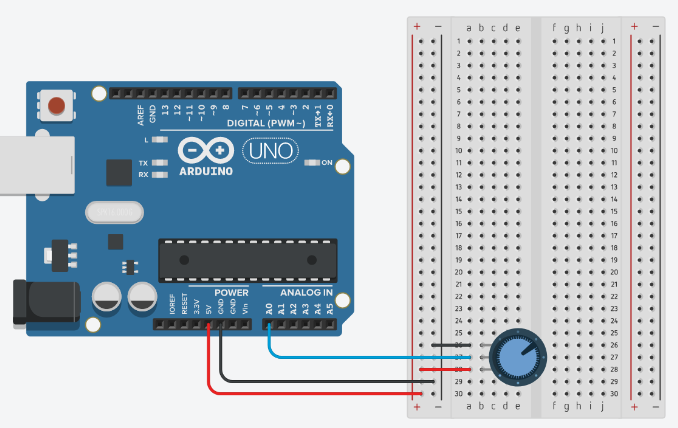
\includegraphics[width=200pt]{01_2_b.png}
    \end{center}

    \subsection*{b)}
    Eg gjer som i øving 1 (oppg. 2c) og finner eit forholdstal for å rekne om til spenning
    \begin{lstlisting}[language=Arduino, basicstyle=\small]
//Rekner ut spenning i A0 og printer til Serial
pinVoltage = potMeterReading * 0.004887586;
Serial.println(pinVoltage);
    \end{lstlisting}
  Det vi måler her er spenningsfallet over den delen av $R_{pot}$ som til ein kvar
  tid befinner seg mellom $A0$ og $5V$.

    \subsection*{c)}
    Tilsvarande som i øving 1 (oppg. 2d) finner eg spenninga vha. spenningsdeling. 
    \begin{lstlisting}[language=Arduino, basicstyle=\small]
const int potMeterPin = A0;
const int potMeterTotalResistance = 10000;

int potMeterReading;
float pinVoltage;
float potMeterResistance;


void setup(){
  pinMode(potMeterPin, INPUT);
  Serial.begin(9600);
  }

void loop() {
  potMeterReading = analogRead(potMeterPin);

  // Calculate voltage from 10 bit value
  //  Constant 0.004887586 is derived from
  //  k = 5V / 1023 (value span)
  pinVoltage = potMeterReading * 0.004887586;

  // Calculate resistance from 10 bit value
  potMeterResistance = potMeterTotalResistance - (pinVoltage * potMeterTotalResistance) / 5;
  Serial.print("voltage: ");
  Serial.print(pinVoltage);
  Serial.print(" resistance: ");
  Serial.println(potMeterResistance);

  delay(10);
}
    \end{lstlisting}
    \newpage

    \subsection*{d)}
    Dette løyste eg med å lage ein funksjon.
    \begin{lstlisting}[language=Arduino, basicstyle=\small]
const int potMeterPin = A0;
const int potMeterTotalResistance = 10000;


int valueToRange(float value, int numOfDivisions, int valueSpan){
  /* Divides valueSpan into numOfDivisionsand check which
   *  division the provided value is in => (0 - numOfDivisions). 
   */
  int valueInRange;
  int division = valueSpan / numOfDivisions;
  
  for (int i = 0; i < numOfDivisions; i++){
    if (value < division * (i+1)){
      valueInDivision = i;
      break;
    }
  }
  return valueInDivision;
}


void setup(){
  pinMode(potMeterPin, INPUT);
  Serial.begin(9600);
  }

void loop() {
  int potMeterReading = analogRead(potMeterPin);

  // Find which range the value is in
  int range = valueToRange(potMeterReading, 4, 1024);

  Serial.println(potMeterReading);
  Serial.println(range);
  
  
  delay(100);
}
    \end{lstlisting}

    \newpage

  \section*{Oppgåve 3 - \textit{analogWrite()} og PWM}
    \subsection*{a)}
    Eg kopler LEDen i serie med ein $220\si{\ohm}$-motstand mellom jord og pin 3.
    \begin{center}
      \begin{circuitikz}[american] \draw
        (0,0) to[full led, *-*] (3,0)
              to[R, l=220<\ohm>, *-*] (6,0)

        (0,0) node[label={[font=\footnotesize]100:$GND$}] {}
        (7,0) node[label={[font=\footnotesize]100:$pin_3$}] {}
        ;
      \end{circuitikz}
    \end{center}


    \begin{lstlisting}[language=Arduino, basicstyle=\small]
#define LED_PIN = 3;

int ledPinState = 0;
bool waveIsRising = true;

void setup(){
  pinMode(LED_PIN, OUTPUT);
}


void loop() {

  // ledPinState triangle wave
  if (waveIsRising) {
    if (ledPinState < 255){
      ledPinState ++;
    } else {
      waveIsRising = false;
    }
  } else {
    if (ledPinState > 0) {
      ledPinState --;
    } else {
      waveIsRising = true;
    }
  }

  analogWrite(LED_PIN, ledPinState);
  delay(5);
}
    \end{lstlisting}
    Denne koden produserer ein jamn triangelbølgeform på pin 3 vha. PWM.
    \newpage


    \subsection*{b)}
    Eg måler motstanden over fotoresistoren og ser at den har eit verdispenn på omtrent
    $30\si{\kilo\ohm}$. Under normal belysning i rommet har fotoresistoren ein motstand
    $1,8\si{\kilo\ohm}$
    \begin{center}
      \begin{circuitikz}[american] \draw
        (0,0) to[photoresistor, l=$R_{fotoresistor}$, *-*] (3,0)
              to[R, l=$R_{E}$, *-*] (6,0)

        (0,0) node[label={[font=\footnotesize]100:$VCC$}] {}
        (3.5,0) node[label={[font=\footnotesize]100:$A0$}] {}
        (7,0) node[label={[font=\footnotesize]100:$GND$}] {}
        ;
      \end{circuitikz}
    \end{center}
    spenninga i A0 er dermed gitt som
    \begin{equation}
      v_{A0} = \frac{R_{fotoresistor}}{R_E + R_{fotoresistor}}5V
    \end{equation}
    Om $R_E$ er for stor eller for liten vil verdispennet i $A0$ gå mot 0. Derfor velger
    eg $R=2\si{\kilo\ohm}$ som eit utgongspunkt sidan det tilsvarar ein verdi ein kan
    forvente i eit normalt opplyst rom.
    \bigskip

    For å tilpasse verdien til lysdioden lager eg meg to skalaer. Botnpunktet til
    fotoresistorverdien setter eg til 150, som er ein verdi det er lett å halde seg under
    når ein blokkerer lyset inn til fotoresistoren med tri fingrar.
    \begin{center}
      \begin{tabular}{ |c|c|c| }
        \hline
        Lysverdi & Lågast & Høgast \\
        \hline
        fotoresistor & 150 & 1023 \\
        \hline
        LED          & 0   & 255 \\
        \hline
      \end{tabular}
    \end{center}
    Til dette kan vi bruke arduinos \textit{map()}-funksjon.

    \begin{lstlisting}[language=Arduino, basicstyle=\small]
  lightSensorReading = analogRead(PHOTORESISTOR_PIN);
  if (lightSensorReading < DARK_THRESHOLD) {
    ledValue = 0;
  } else {
    ledValue = map(lightSensorReading, DARK_THRESHOLD, 1023, 0, 255);
  };
    \end{lstlisting}
    
    \begin{center}
      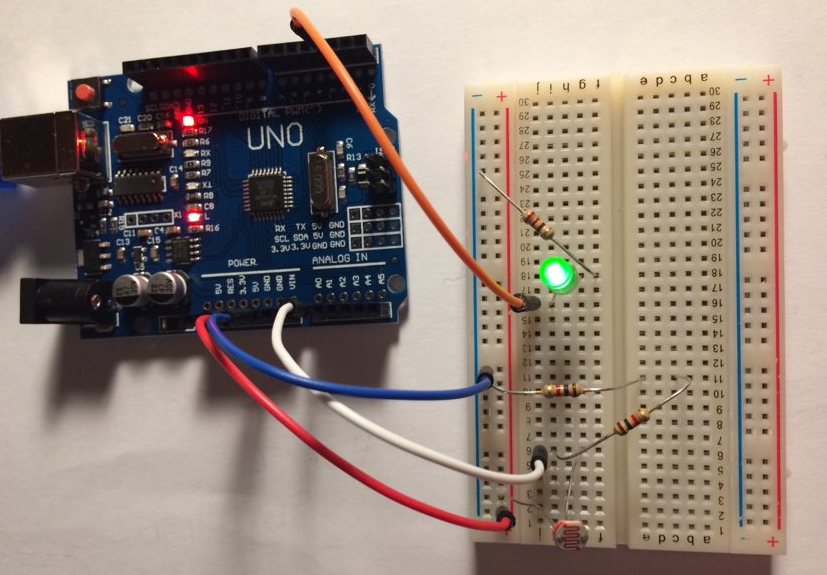
\includegraphics[width=200pt]{02_3_b.png}
    \end{center}

  \newpage

  \section*{Oppgåve 4 - Random}
    \subsection*{a)}
    \begin{lstlisting}[language=Arduino, basicstyle=\tiny]
#define RANDOM_SEED_PIN 2 // Pin 0 must not be used

int randomNumber;

void setup(){
  Serial.begin(9600);  
  randomSeed(analogRead(RANDOM_SEED_PIN));
}

void loop(){
  randomNumber = random(1,7);

  Serial.println(randomNumber);
  delay(1000);
}
    \end{lstlisting}

    \subsection*{b)}
    Eg velger å bruke \textit{random}-generatoren på ein litt annan måte.
    \begin{lstlisting}[language=Arduino, basicstyle=\tiny]
const int randomSeedPin = 2; // This pin must remain unused
const int buzzerPin = 3;
const int fundamentalFreq = 10;
const int toneDuration = 100;


int randomTone;
int currentFreq;


void setup(){
  Serial.begin(9600);  
  randomSeed(analogRead(randomSeedPin));
  pinMode(buzzerPin, OUTPUT);
}


void loop(){
  /* Plays randomly generated music on a piezoelectric buzzer.
   *  The default fundamental frequency of 10 Hz puts about 10-20%
   *  of the notes generated below the audible range, which makes sounds
   *  reminiscent of drums.
   */
  randomTone = random(1,13);

  // Random pure intonation harmonics based on random integer
  currentFreq = fundamentalFreq * randomTone;

  tone(buzzerPin, currentFreq, toneDuration);
  Serial.println(currentFreq);
  delay(toneDuration);
}
    \end{lstlisting}
    \begin{center}
      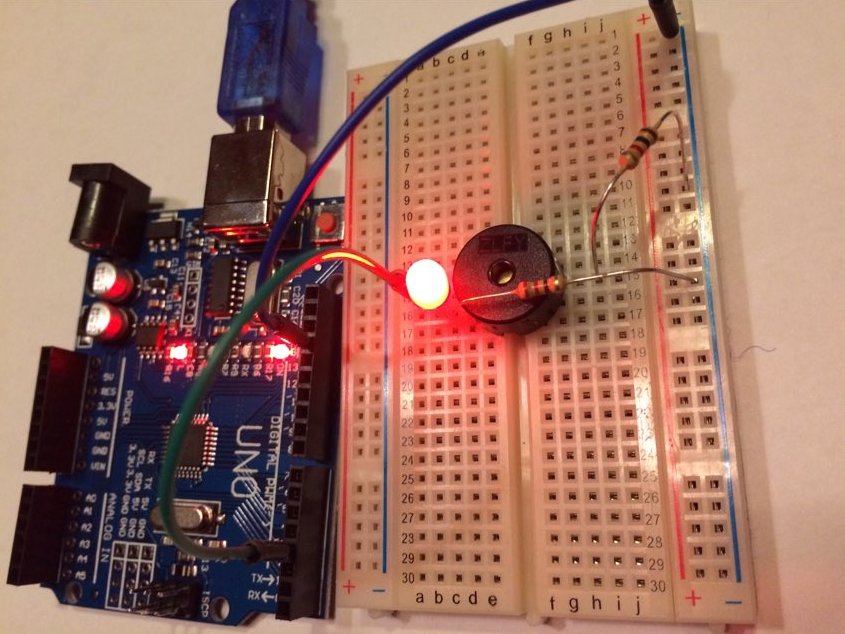
\includegraphics[width=170pt]{02_4_b.png}
    \end{center}

    \subsection*{c)}
    Dette løyste eg på denne måten.

    \begin{lstlisting}[language=Arduino, basicstyle=\small]
const int randomSeedPin = 2; // This pin must remain unused
const int testDuration = 10000;

int randomToss;
int tossAmounts[6];
char strBuf[64];

void setup(){
  Serial.begin(9600);  
  randomSeed(analogRead(randomSeedPin));
}


void loop(){
  // Perform a test of the random generator
  for (int i=0; i<testDuration; i++){
    randomToss = random(0,6);
    tossAmounts[randomToss]++;
  }

  // Print the test results
  sprintf(strBuf, "Test concluded after %d iterations", testDuration);
  Serial.println(strBuf);
  for (int i = 0; i < 6; i++){
    sprintf(strBuf, " num %d: ", i+1);
    Serial.print(strBuf);
    Serial.println(tossAmounts[i]);
  }

  // Reset the tossAmounts array
  memset(tossAmounts, 0, sizeof(tossAmounts));

  delay(1000);
}
    \end{lstlisting}
    Dersom eg ville hatt svara som prosent ville eg gjort om
    \begin{lstlisting}[language=Arduino, basicstyle=\small]
    Serial.println(tossAmounts[i] / testDuration);
    \end{lstlisting}


    \subsection*{d)}
    Først implementerte eg ein versjon med \textit{delay}-kall:
    \begin{lstlisting}[language=Arduino, basicstyle=\tiny]
const int randomSeedPin = 2; // This pin must remain unused
const int buttonPin = 4;
const int testDuration = 10000;

int randomToss;
int tossAmounts[6];
char strBuf[64];


void buttonWait(int pin){
  bool isPressed;
  
  for (;;){
    isPressed = digitalRead(pin);
    if (isPressed) {
      break;
    }
    delay(10);
  }
}


void setup(){
  Serial.begin(9600);  
  randomSeed(analogRead(randomSeedPin));
  pinMode(buttonPin, INPUT);
}


void loop(){
  // Wait for user to press button
  Serial.println("Press button to perform test.");
  buttonWait(buttonPin);
  Serial.println("   testing...");
  
  // Perform a test of the random generator
  for (int i=0; i<testDuration; i++){
    randomToss = random(0,6);
    tossAmounts[randomToss]++;
  }
  
  // Print the test results
  sprintf(strBuf, "Test concluded after %d iterations", testDuration);
  Serial.println(strBuf);
  for (int i = 0; i < 6; i++){
    sprintf(strBuf, " num %d: ", i+1);
    Serial.print(strBuf);
    Serial.println(tossAmounts[i]);
  }
  
  // Reset the tossAmounts array
  memset(tossAmounts, 0, sizeof(tossAmounts));
}
    \end{lstlisting}
    Når eg implementerte trykknappkretsen vart eg klar over problemet med knappeprell.
    Ein måte å løyse dette på som har mange andre fordelar er å implementere programmet
    vha. separate tilstandsmaskiner. Eg teikna eit tilstandsdiagram for knappen som tar
    hensyn til at transienten har mykje støy dei første 5 millisekunda.

    \begin{center}
      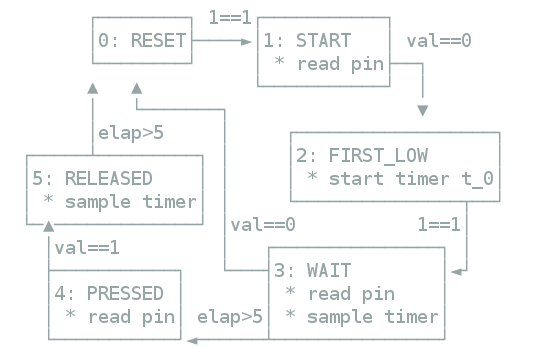
\includegraphics[width=170pt]{02_4_d.png}
    \end{center}
    Dette implementerte eg på denne måten:
    \begin{lstlisting}[language=Arduino, basicstyle=\tiny]
#define BUTTON_1_PIN 6
#define BUTTON_2_PIN 5
#define BUTTON_3_PIN 4

const bool WRITE_TO_SERIAL = true;

class ButtonStateMachine {
  /* Button state machine class with debouncing
   *  on both push and release transients.
   *  Pull down switch: vcc--[SWITCH]--sample--[R=220]--gnd */
  private:
    bool val;
    uint8_t pin;
    unsigned long t;
    unsigned long t_0;
    const uint8_t bounce_delay = 5;
    
  public:
    uint8_t state_prev = State::RESET;
    bool state_has_changed;
    
    enum State : uint8_t {
      RESET = 0,
      START,
      FIRST_LOW,
      WAIT,
      PRESSED,
      RELEASED
    };
    State state = State::RESET;

    ButtonStateMachine(uint8_t pin) {
      this->pin = pin;
      Init();
    }

    void Init(){
      pinMode(pin, INPUT);
    }
    
    void NextState(){
      state_prev = state;
      
      switch (state){
        case State::RESET:
          state = State::START;
        break;
    
        case State::START:
          val = digitalRead(pin);
          if (val == LOW) {state = State::FIRST_LOW;}
        break;
    
        case State::FIRST_LOW:
          t_0 = millis();
          state = State::WAIT;
        break;
    
        case State::WAIT:
          val = digitalRead(pin);
          t = millis();
          if (val == LOW) {state = State::RESET;}
          if (t - t_0 > bounce_delay){state = State::PRESSED;}
        break;
    
        case State::PRESSED:
          val = digitalRead(pin);
          t_0 = millis();
          if (val == HIGH) {state = State::RELEASED;}
        break;
    
        case State::RELEASED:
          t = millis();
          if (t - t_0 > bounce_delay){state = State::RESET;}
        break;
      }
      state_has_changed = (state_prev != state);
    }
};


// Global object instantiations
ButtonStateMachine button_1(BUTTON_1_PIN);
ButtonStateMachine button_2(BUTTON_2_PIN);
ButtonStateMachine button_3(BUTTON_3_PIN);


void setup(){
  if (WRITE_TO_SERIAL) {Serial.begin(9600);}
}


void loop(){
  button_1.NextState();
  button_2.NextState();
  button_3.NextState();

  // Debug
  if (WRITE_TO_SERIAL) {
    if (button_1.state_has_changed){
      if (button_1.state == ButtonStateMachine::State::PRESSED) {Serial.println("BUTTON ONE");}
      Serial.print(" state_s1: ");
      Serial.println(button_1.state);
    }
    if (button_2.state_has_changed){
      if (button_2.state == ButtonStateMachine::State::PRESSED) {Serial.println("BUTTON TWO");}
      Serial.print(" state_s2: ");
      Serial.println(button_2.state);
    }
    if (button_3.state_has_changed){
      if (button_3.state == ButtonStateMachine::State::PRESSED) {Serial.println("BUTTON THREE");}
      Serial.print(" state_s3: ");
      Serial.println(button_3.state);
    }
  }
}
    \end{lstlisting}

    Dette designmønsteret har mange fordelar
    \begin{itemize}
      \item Det er nå mogleg å ha fleire samtidige prosessar, i motsetning til om ein bruker
        \textit{delay}-kall
      \item Systemet har ein endeleg mengde tilstandar, noko som gjer det mogleg å rapportere
        heile systemets tilstand i korte trekk.
      \item Dette gjer det også lettare å lese av ein tidsbruksprofil av systemet for å 
        optimalisere overgangane og gjere systemet raskare.
      \item Sidan \textit{ButtonStateMachine} er ein objektdefinisjon er det lett å gjenbruke
        koden og instansiere så mange knappeobjekter ein vil.
    \end{itemize}

\end{document}
